% introduction secion of the main paper
% it sets the context of our research and explains the goal of the paper
\section{Context}

	Many works of art deteriotate significantly over time.

	From an artistic point of view, it is of much interest to be able to view the drawings
	in the original coloring or, as one might say: in the way the artist intended the drawing.
	Paintings are often treated by curators to remove some of the pollution and regain
	the original properties.  Other works of art, of which the original is not recoverable by
	treating or cleaning the original piece (such as ink drawings), can be reproduced.
	Either on paper or digitally. \\

	Both of these recovery processes are time intensive and require a specialist's hand.
	And, when treating the original, it poses a risk of damaging the piece. \\

	We will specifically examine the recovery of the original coloring of ink drawings.
	Several types of detoriation occur with ink drawings:

	\begin{itemize}
		\item ink bleeding through from the backside of the drawing to the front
		\item ink color fading, due to light exposure
		\item paper decoloration, due to light exposure
	\end{itemize}

	The effects of above mentioned processes can be quite dramatic, as can be seen from
	figure \ref{montmajour}.

	\begin{figure}[h!]
		\label{montmajour}
		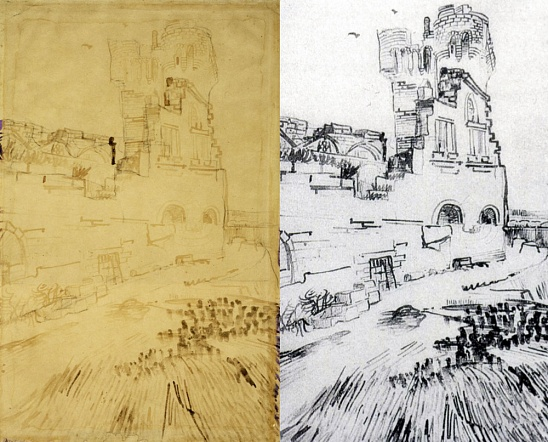
\includegraphics[width=\columnwidth]{graphics/montmajour}
		\caption{Reproduction of 'Montmajour' by Vincent van Gogh (1928) and a photographic reproduction}
	\end{figure}

	One might wonder how the original colors of a work can be determined.
	There are several sources that can tell us what the original colors where:

	\begin{itemize}
		\item margins of a drawing that were obscured from light by the frame
		\item (photographic) reproductions and/or facsimiles of the drawing
		\item similar drawings, of the same theme, same period
                  or made with the same ink % on the same paper?
	\end{itemize}

\section{Introduction}

	As mentioned before, the original can be reproduced digitally.
	A lot of time could potentially be saved if digital imaging techniques can be used to automate
	the recoloring of degraded work to the original colors.
	In the imaging field, a lot of techniques have been developed for retrieving information
	from images, recognizings patterns and color adjustments.
	Most of these techniques were not developed with art restauration as it's goal.
	Our research focusses on applying these existing methods to this specific problem. \\

	In this article we will examine a few of these techniques.
	We will discuss how these techniques can be applied to recover the original colors
	in faded ink drawings.
	Furthermore we will compare the techniques and based on that discussion formulate a possible
	method for digital reconstruction.
